\documentclass[UTF8]{csoarticle}


\newtheorem{theorem}{定理}
\newtheorem{lemma}{引理}
\renewcommand{\proofname}{证明}
% 如果为英文文章,可以使用下面的定义(去除行首的注释符号%)代替上述中文定义
% \newtheorem{theorem}{Theorem}
% \newtheorem{lemma}{Lemma}

\begin{document}

%----------------------------------------------------------
% 1. 文章标头信息
%----------------------------------------------------------

\titleCHN{基于局部特征的图像重建算法}
\titleENG{Image Reconstruction Based on Local Features}
\authorCHN{王继哲\affil{1},李学明\affil{2}}
\authorENG{WANG Ji-Zhe\affil{1}, LI Xue-Ming\affil{2}}
\affiliationCHN{
    \affil{1} 北京邮电大学信息与通信工程学院,北京 100876 \\
    \affil{2} 北京邮电大学信息与通信工程学院,北京 100876
}
\affiliationENG{
    \affil{1} School of Information and Communication Engineering, Beijing University of Posts and Telecommunications, Beijing 100876 \\
    \affil{2} School of Information and Communication Engineering, Beijing University of Posts and Telecommunications, Beijing 100876
}

\abstractCHN{综述文章:以背景、研究现状、研究用途的结构书写,篇幅以150~300字左右为宜,不用第一人称做主语,不与正文语句重复。一般研究性文章:以摘录要点的形式按目的、方法、结果、结论的结构报道出作者的主要研究成果,字数在200~400字左右为宜,不用第一人称做主语,不与正文语句重复。
基于局部特征的图像重建算法是利用原始图像的局部特征信息,以大图像集为数据源,进行较为精确的图像重建工作,使重建后的图像与原始图像相似,并且图像质量达到人眼主观效果较好的程度。本文首先对目前图像重建算法加以概述,综合介绍重建系统中的局部特征、视觉词组、相似图像搜索、特征匹配、特征配准、匹配特征块筛选、图像融合等多种计算机视觉相关技术。之后将该系统引入大语料集的应用场景下,对上述几个环节进行完善,主要包括在(1)相似搜索环节引入GEO-Hash索引技术并提出分块相似搜索,一方面极大加快了搜索速度,另一方面提高了搜索结果的多样性;(2)在匹配块筛选法中提出阈值自适应的验证准则。为匹配块的筛选提供更有力的依据,显著提升了拼接结果。}

\abstractENG{abstract text}
\keywordCHN{中文关键词要能反映文章的基本观点,避免广义词。第一个关键词为该文内容所属二级学科名称}
\keywordENG{list of keywords}
\cateidCHN{请查阅《中国图书馆分类法》}

\authorIntroduction{王继哲(1989-),男,硕士研究生,主要研究方向:多媒体通信,图像处理。通信作者:李学明(1969-),男,教授,主要研究方向:多媒体通信,图像处理。}
\fund{***基金(00000000),***基金(00000000)}

\maketitle


%----------------------------------------------------------
% 2. 正文内容
%----------------------------------------------------------

\section{引言}

简要回顾研究工作的背景和研究目的,一般400~600字,不超过800字。

随着移动终端计算能力的提升,终端应用迎来蓬勃发展,图片类应用日益普及,每天有数以万计的高分辨率图像由移动终端上传到服务器上,给通信网络带宽造成了巨大的压力。
另一方面我们观察到随着存储设备容量变大、芯片计算能力的提升,互联网用户的不断增多,大数据时代来临。图像数据数以亿计,服务器计算能力极大提升。从信息的角度来说,我们拍摄的每一幅图像中所包含的部分或全部内容都可以在互联网上其它图像中找到。

在2013年有学者[文献6]提出一种全新的压缩方式——基于云的图像编码。其核心思想是在客户端提取并编码发送少量的图像特征数据,并不传输图像数据本身,而在服务器端解码后利用特征数据在服务器的大图像数据集上匹配相似的图像,利用相似图像进行图像的重建。这种架构所运用的核心技术手段便是基于局部特征的图像重建算法。系统的核心思想是通过对原始图像的特征提取与重建,利用计算资源减少带宽损耗,从一个全新的维度进行数据压缩,为多媒体应用开启了一扇大门。

图像重建任务的核心是通过局部特征找到与原始图像相似的图像单元以及可靠的图像间对应点集合,进而自动地建立图像之间点与点或区域与区域之间的可靠对应关系,根据对应关系采用一定的算法拼接图像单元。基于局部特征对图像进行重建的技术能够让我们在发送端只传输少量的特征数据,而接收端服务器利用大数据集进行高分辨率图像的还原。

本文在上述的大框架下综合使用多种信息检索与图像处理技术,对其中的相似图像检索、图像块筛选等核心算法进行了改进与完善,使之更加能够适用于大规模图像集上的图像重建任务,重建速度得到提升,重建结果得到了进一步的优化。

\section{基于局部特征的图像重建算法}
在本文的应用场景下,图像重建的部分流程可以看成是多幅图像的全景图拼接问题。与文献\cite{Brown:2006ir}中的流程类似,主要包含以下几个环节:(1)使用具有不变性的特征来描述图像;(2)自动的找到图像之间的空间位置关系,进行图像配准;(3)图像融合,消除不同图像之间的光照差别,去除边缘噪声。与全景图拼接不同的是,本文提出的图像重建系统每幅小图(Patch)块大小不一,导致图像空间位置关系可能存在不准确,多幅图像之间有大量重叠,整体思路是先融合大块,后融合小块,分别介绍如下。

\subsection{图像的局部特征}
图像的局部特征是计算机视觉领域一个基本问题,它能够反映图像某一局部的特性,对寻找图像对应的局部单元以及特征描述中有着重要作用。通常意义的局部特征包含两个方面,特征检测子(Detector)和特征描述子(Descriptor)。检测子能够检测出我们“感兴趣”的点或者局部区域,而一个好的局部特征描述子反映出图像的局部特性能够帮助找到图像与图像点集合对应关系,进而建立图像之间的空间对应关系。局部图像特征描述的核心问题是不变性(invariant)和可区分性(discrimination)。

在多种局部特征中,本文选择使用Lowe提出的尺度不变特征变换(Scale Invariant Feature Transform,以下简称SIFT)。SIFT算子是图像局部特征研究领域的一项重大突破。SIFT算子具有很强的可区分性,同时对尺度、旋转以及一定视角和光照变化等图像变化都具有不变性。

\subsubsection{尺度空间理论}
尺度空间是模拟图像数据的多尺度特征:尺度空间中图像的模糊程度逐渐变大,能够模拟人在距离目标由近到远时目标在视网膜上的成像过程。我们可以把两幅图像想象成是连续的,分别以它们作为底面作四棱锥,就像金字塔,那么每一个截面与原图像相似,金字塔的两层中包含无穷个截面,在实际应用只能选择离散诘责,构造有限个层。一个图像的尺度空间,\(L(x,y,\sigma)\)定义为一个变化尺度的高斯函数\(G(x,y,\sigma)\)与原图像\(I(x,y)\)的卷积。
\begin{align}
  L(x,y,\sigma) = G(x,y,\sigma) \otimes I(x,y)
\end{align}


\section{一些格式说明}

\subsection{正文}

\subsubsection{正文字体}

当需要强调某些文字时,建议使用 \verb|\emph{文字}| 命令,也可以直接使用 \verb|\textbf{加粗文字}| 或 \verb|\textit{倾斜文字}| 等。

\subsubsection{脚注}

在正文中插入脚注使用 \verb|\footnote{脚注文本}| 命令\footnote{这里放置脚注的文本内容。}。

\subsubsection{参考文献引用}

在正文中引用参考文献使用序号方式,并根据上下文确定文献引用序号是否采用上标方式。举例:在文献\cite{bib1}中提出一种方法,后续研究对该方法进行了改进\upcite{bib1,bib2}。

\subsection{图形}

本模板提供的文档类 \verb|csoarticle| 本身默认情况下已经包含了 \verb|graphicx| 宏包,因此典型方法是用 \verb|\includegraphics| 命令将图形包含到浮动环境 \verb|figure| 中。图 \ref{fig:sample} 是一个例子。除了 \verb|pdf| 格式外,也支持 \verb|eps|, \verb|jpeg| 等多种格式,具体用法可参看 \verb|graphicx| 宏包的文档。
\begin{figure}
\centering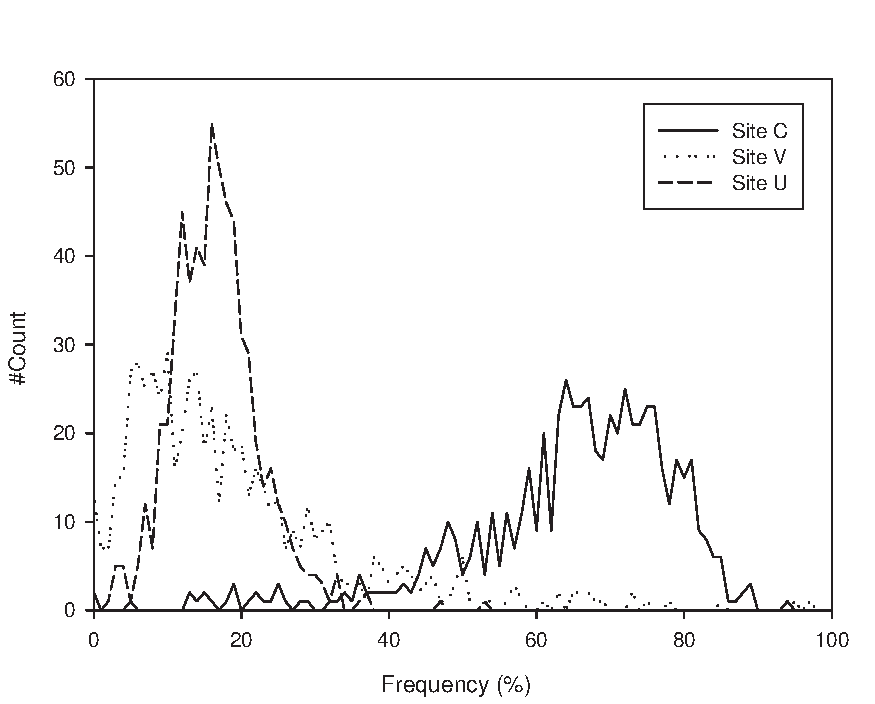
\includegraphics[height=6cm]{figsamp}
\caption{数据曲线图示例}
\label{fig:sample}
\end{figure}

\subsection{表格}

使用浮动环境 \verb|table| 的示例见表\ref{tab:sample}。
\begin{table}
  \caption{表格示例}
  \label{tab:sample}
  \centering
  \begin{tabular}{lcr}%{|l|c|r|}
    \hline
    求解算法                & 系数矩阵的规模    & 执行时间(秒)  \\
    \hline
    Gauss消去法(直接法)     & Mat1903           &  113.27       \\
    Jacobi点迭代            & Mat1784           &  201.36       \\
    \hline
  \end{tabular}
\end{table}

\subsection{数学公式}

本模板提供的文档类 \verb|csoarticle| 本身默认情况下已经包含了 \verb|amsmath| 和 \verb|amsthm| 宏包,因此可以使用这些宏包中提供的一切命令。带编号的数学公式建议使用 \verb|align| 环境。举例如下:一元二次方程
\begin{align}\label{eq:sample}
    a x^2 + b x + c = 0
\end{align}
的两个根为
\begin{align}\label{eq:root}
    x_1 &= \frac{-b + \sqrt{b^2 - 4ac}}{2a} \\
    x_2 &= \frac{-b - \sqrt{b^2 - 4ac}}{2a}
\end{align}
其中,方程\eqref{eq:sample}中的系数$a \not= 0$。

数学类内容中常用的定理类环境也可以直接使用,举例如下(\emph{均为虚拟例子,切勿进行技术性探究}):
\begin{lemma}\label{lem:levy}
    引理的具体内容。
\end{lemma}
\begin{proof}
    可参看各类数学分析类教材,此处从略。
\end{proof}

\begin{theorem}[牛顿第二定律]\label{thm:newton}
物体的质量$m$、物体所受的力$F$以及物体运动的加速度$a$之间满足
\begin{align}\label{eq:f-eq-ma}
    F = m a
\end{align}
\end{theorem}
\begin{proof}
由引理\ref{lem:levy}及文献\cite{bib1}第15章的定理4可立得。
\end{proof}

请直接查看以上例子的源代码部分。

\subsection{参考文献的格式要求}

文献数量应不低于6篇,综述文章文献数量不低于25篇。

注:文中所引的参考文献, 作者均应认真阅读过, 对文献的作者、题目、发表的刊物、年份、卷期号和起止页码等均应核实无误,并按在正文出现的先后顺序编号。标引的序号两边加“[ ]”,作者不超过3人的姓名都写, 超过3人的第三人后面加“,等(et al)” 。无论中外署名,一律姓(大写)先名后,作者姓名之间以逗号分隔。参考文献一律置于文末。文献正文中所有非英文文献需写出对应的英文译文,具体格式要求如下(例子请参看本模板文后的参考文献):
\begin{enumerate}
\item\textbf{期刊:}     作者. 论文题目[J]. 刊名,年,卷(期):起始页码~终止页码.
\item\textbf{专著:}     作者. 书名[M]. 出版地:出版社,出版年.
\item\textbf{译著:}     作者. 书名[M]. 译者. 出版地:出版社,出版年.
\item\textbf{论文集:}   作者. 论文题目[A]. 编者. 文集[C]. 出版地:出版社,出版年. 起始页码~终止页码.
\item\textbf{学位论文:} 作者. 论文题目[D]. 所在城市:保存单位,年份.
\item\textbf{技术标准:} 起草责任者,技术标准代号顺序号—发布年. 技术标准名称[S]. 出版地:出版社,出版年.其中,起草责任者、出版地、出版社、出版年可省。
\item\textbf{专利:}     申请者. 专利名[P]. 国名及专利号,发布日期.
\item\textbf{技术报告:} 作者. 文题[R]. 地名:责任单位,报告代码及编号,年份.
\item\textbf{报纸文章:} 作者. 文题[N]. 报纸名,出版日期(版次).
\item\textbf{在线文献:} 作者. 文题[OL]. [日期]. http://......
\item\textbf{光盘文献:} 作者. 文题[CD]. 出版地:出版者,出版日期.
\item\textbf{其他文献:} 作者. 文题[Z]. 出版地:出版者,出版日期.
\end{enumerate}

\section{结论}

本文给出了………

\section*{致谢(可选)}

应向对论文有帮助的有关人士或单位表示谢意。


%----------------------------------------------------------
% 3. 参考文献
%----------------------------------------------------------

\begin{thebibliography}{2} % 这里的2是指参考文献总数目,需要根据实际情况进行修改
    \bibitem{bib1} H.E.S.Said, T.Tan and K.Baker.Personal identification based on handwriting [J].Pattern Recognition, 33:149-160, Jan. 2000
    \bibitem{bib2} 吴佑寿,丁晓青.汉字识别原理与应用[M],北京:高等教育出版社,1992.8
\end{thebibliography}

\end{document}
